

\begin{figure*}
    \centering
    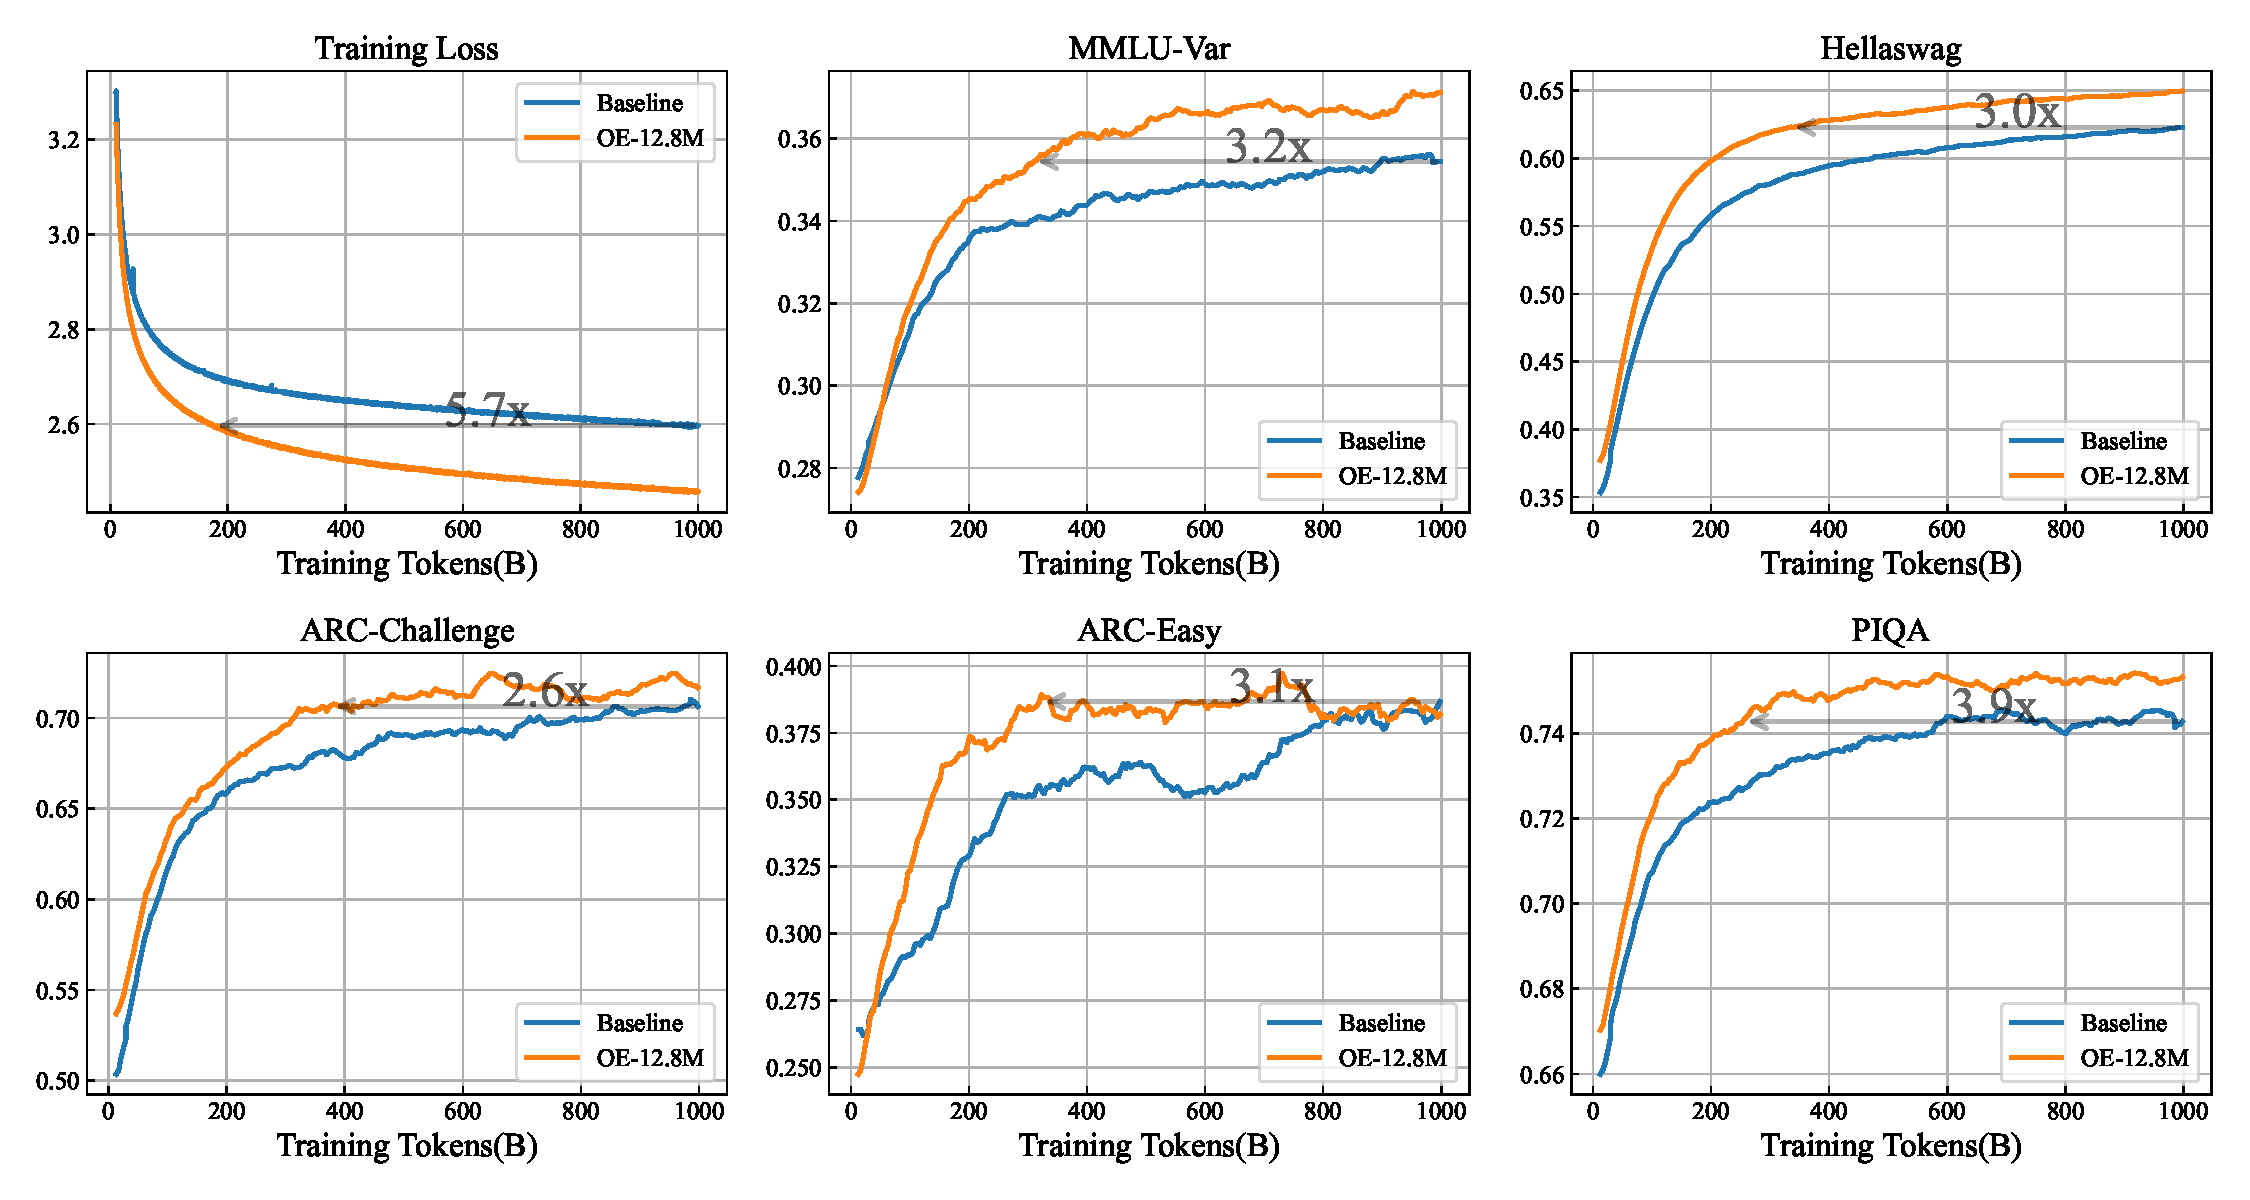
\includegraphics[width=0.96\linewidth]{figures/olmo2_1T_1B_acceleration.pdf}
    \caption{Training curves for OE-12.8M and baseline model on OLMo2-1B. The metrics are smoothed via exponential moving average with weight 0.99 for loss and 0.9 for downstream tasks. We observe significant convergence acceleration for the OE model: $5.7\times$ on loss, $3.2\times$ on MMLU-Var, $3.0\times$ on Hellaswag, $2.6\times$ on ARC-Challenge, $3.1\times$ on ARC-Easy and $3.9\times$ on PIQA. }
    \label{fig:olmo2_1B_training_dynamics}
\end{figure*}


\section{Experiments}

\paragraph{Implementation.} Our experiments focus on large language modeling tasks and basically follow OLMo series works. We maintain the training configuration of baseline model, replacing the word embedding with over-encoding technique. The original tokenizer used in baseline models is preserved as the base tokenizer in our method. The experiments are run with engineering optimized implementation. 
We refer OE-$m$ to over-encoded models with $m\times d_{model}$ embedding parameters in total. Typically, we implement with $n=3, m=1.28\times10^7$, \ie OE-12.8M, and variate $k$ according to $d_{model}$, making $\frac{d_{model}}{nk}\approx 256$. 

\paragraph{Metrics.} We report the average perplexities (PPL) and losses on the \texttt{c4\_en-validation} dataset as the `Eval PPL' or `Eval Loss', along with the metrics for zero-shot evaluation on downstream benchmarks. We observe significant volatility in the zero-shot performance indicators for the datasets. For more reliable and consistent results, we mainly concern five stable tasks in our analysis: MMLU-Var, Hellaswag, ARC-Challenge, ARC-Easy and PIQA. Detailed descriptions on these tasks and more comprehensive evaluations can be found in Appendix~\ref{sec:appendix_more_exps}.

\subsection{Over-Encoding Scaling Trend}

\paragraph{Dense Models}
We follow the experimental setup described in OLMo2~\cite{olmo20242olmo2furious}, which is currently the state-of-the-art fully open model. We maintain most of the training configurations, but modify the architecture to obtain models with 151M, 400M and 1B dense parameters, which is denoted by OLMo2-151M, OLMo2-400M and OLMo2-1B, respectively. We train OLMo2-151M and OLMo2-400M models with 400B tokens, and OLMo2-1B with 1T tokens. In addition to OE-12.8M models, we also run experiments for OE-1.2M to offer a rough scaling trend on vocabulary size.

The result is ploted in \figref{fig:model_size_scaling}. From comparisons across model scales, OE models hold consistent improvements from baseline models. Specifically, the OE-12.8M model achieves comparable performance to a baseline model that is 2.5 times larger in model scale (comparing the 400M OE model with the 1B baseline model). Moreover, the vocabulary size of OE-12.8M, OE-1.2M, and the baseline model (vocabulary size $V=100278$) exhibits exponential growth, while their scaling curves maintain approximately equal spacing. This observation suggests a log-linear relationship between vocabulary size and model performance, which we further validate in the ablation studies.

We present the training dynamics for OLMo2-1B models in \figref{fig:olmo2_1B_training_dynamics}. Compared to the baseline model, OE demonstrates consistently increasing performance gains, with an improvement of 0.12 at 400B tokens that expands to 0.14 at 1T tokens. From the perspective of convergence acceleration, training loss achieves a remarkable 5.7$\times$ speedup. Furthermore, in terms of downstream evaluation, OE exhibits substantial acceleration, achieving 3.2$\times$, 3.0$\times$, 2.6$\times$, 3.1$\times$ and 3.9$\times$ speedups on MMLU-Var, Hellaswag, ARC-Challenge, ARC-Easy and PIQA, respectively. A thorough evaluation is ploted in Appendix~\ref{sec:appendix_detailed_olom2_exps}.



\begin{table}
\centering
\caption{Performance of Over-Encoding on MoE architecture with 500B tokens' training. The column `Emb. P.' represents `Embedding Parameters'. `Downstream' stands for the average of MMLU-Var, Hellaswag, ARC-Challenge, ARC-Easy, and PIQA. For `+OE' rows, we provide metric difference with blue labels.}
\resizebox{\columnwidth}{!}{%
\begin{tabular}{lc|ll}
\toprule
Model & \# Emb. P. & Loss$\downarrow$ & Downstream$\uparrow$ \\ 
\midrule
OLMoE-1.3B & 51M & 2.554 & 0.510 \\
+OE-12.8M & 13.1B & 2.472 \scriptsize \textcolor{blue}{-0.082} & 0.524 \scriptsize \textcolor{blue}{+0.014} \\
\hline
OLMoE-7B & 102M & 2.305 & 0.601 \\
+OE-12.8M & 26.3B & 2.229 \scriptsize \textcolor{blue}{-0.076} & 0.608 \scriptsize \textcolor{blue}{+0.007} \\
\bottomrule
\end{tabular}%
}
\label{tab:olmoe_sota_oe}
\end{table}

\paragraph{MoE Models}
Sparse Mixture-of-Experts (MoE) models~\cite{shazeer2017} have also achieved great success in recent years. These models aim to introduce sparse Feed-Forward Network (FFN) modules, enabling the addition of a large number of sparse parameters to improve model performance while keeping the same number of activated parameters, making the training and inference costs unchanged. Similarly, we evaluate the effectiveness of OE under the MoE architecture.

We follow the experimental setup described by OLMoE~\cite{muennighoff2024olmoeopenmixtureofexpertslanguage}. In the experiments, OLMoE-1.3B refers to a model with 260M active parameters and a total of 1.3B parameters, while OLMoE-7B refers to models with 1.3B active parameters and a total of 7B parameters. In this setting, the base tokenizer has vocabulary size $V=50280$, and we train 500B tokens for all these models.

The results are shown in \tabref{tab:olmoe_sota_oe}. We first compare the training loss. At two different model scales, OE-12.8M achieves approximately the same improvement in loss compared to the baseline, despite decreases in the proportion of embedding parameters as the model scales up (\ie, 10$\times$ dense parameters for OLMoE-1.3B and 3.7$\times$ for OLMoE-7B). However, in terms of downstream evaluation metrics, the performance improvement of OE diminishes. We hypothesize that this reduction is related to the sparse parameters utilized in the MoE architecture, which may overlap with the benefits provided by sparse embedding parameters.

\begin{table*}[h!]
\centering
\renewcommand{\arraystretch}{1.3}
\setlength{\tabcolsep}{3.5pt}
\caption{Ablation study on different input vocabulary designs. The downstream tasks follow the eval settings in OLMoE, where MMLU-V stands for MMLU-Var, HS for Hellaswag, ARC-C for ARC-Challenge and ARC-E for ARC-Easy. All models are trained with 500B tokens.}
\label{tab:over_enc_good_exps}
\begin{tabular}{@{}llcccccccccc@{}}
\toprule
\multirow{2}{*}{Id} & \multirow{2}{*}{Model} & \multicolumn{2}{c}{Train} & \multicolumn{2}{c}{Eval} & \multicolumn{5}{c}{Downstream} \\ 
\cmidrule(lr){3-4} \cmidrule(lr){5-6} \cmidrule(lr){7-11}
& & Loss$\downarrow$ & PPL$\downarrow$ & Loss$\downarrow$ & PPL$\downarrow$ & MMLU-V$\uparrow$ & HS$\uparrow$ & ARC-C$\uparrow$ & ARC-E$\uparrow$ & PIQA$\uparrow$ \\ 
\midrule
1 & OLMoE-1.3B & 2.554 & 12.864 & 2.924 & 18.625 & 0.327 & 0.553 & 0.325 & 0.622 & 0.727 \\ 
2 & +$\mathbb{E}^{3.2\mathrm{M}\times d}(x^{(-2)})$ & 2.511 & 12.319 & 2.887 & 17.944 & 0.340 & 0.569 & \textbf{0.351} & \textbf{0.656} & 0.734 \\ 
3 & +$\mathbb{E}^{6.4\mathrm{M}\times \frac{d}{2}}(x^{(-2)})$ &2.507 & 12.268 & 2.882 & 17.851 & 0.330 & 0.573 & 0.341 & 0.648 & 0.731 \\ 
4 & +$\mathbb{E}^{3.2\mathrm{M}\times d|2}(x^{(-2)})$ & 2.503 & 12.221 & 2.877 & 17.754 & 0.337 & 0.575 & 0.345 & 0.651 & \textbf{0.740} \\ 
5 & +$\mathbb{E}^{3.2\mathrm{M}\times d|4}(x^{(-2)})$ & 2.503 & 12.226 & 2.876 & 17.736 & 0.328 & 0.575 & 0.337 & 0.653 & 0.734 \\ 
6 & +$\sum_{i\in\{2,3\}}\mathbb{E}_i^{3.2\mathrm{M}\times \frac{d}{2}|2}(x^{(-i)})$ &\textbf{2.495} & \textbf{12.127} & \textbf{2.870} & \textbf{17.638} & \textbf{0.340} & \textbf{0.578} & 0.330 & 0.636 & 0.738 \\  
\hline 
7 & +$\mathbb{E}^{12.8\mathrm{M}\times d}(x^{(-2)})$ & 2.493 & 12.100 & 2.881 & 17.832 & 0.334 & 0.569 & \textbf{0.343} & 0.643 & \textbf{0.730} \\ 
8 & +$\sum_{i\in\{2,3\}}\mathbb{E}_i^{12.8\mathrm{M}\times \frac{d}{2}|2}(x^{(-i)})$ & \textbf{2.472} & \textbf{11.854} & \textbf{2.862} & \textbf{17.494} & \textbf{0.342} & \textbf{0.577} & 0.329 & \textbf{0.645} & 0.728  \\ 
\bottomrule
\end{tabular}
\end{table*}


\subsection{Ablation Study}

We conduct ablation study basing on the setup of OLMoE-1.3B. To save computational resources, for ablation variants that are non-promising, we only train for 50B tokens. Otherwise, we train for 500B tokens to obtain solid conclusions.



\paragraph{Vocabulary Size Scaling.}
We first analyze the scaling behavior of over-encoding based. Specifically, we use the simplest over-encoding setup with fixed $n=2$ and $k=1$, while varying the value of $m$. The size of $m$ ranges from $20\mathrm{K}$ to $12.8\mathrm{M}$. We train on $500\mathrm{B}$ tokens and evaluate the model performance. As shown in the figure, the experimental results reveal a logarithmic linear relationship between the training loss and $m$: for every $4\times$ increase in $m$, the training loss decreases by 0.015. Finally, we extracted the loss at 500B tokens and plotted the scaling curve shown in \figref{fig:input_vocab_scaling}. Here, the input vocabulary size is defined as the sum of the sizes of the 1-gram and 2-gram vocabularies, i.e., $V + m$. It is worth noting that the model needs to be sufficiently trained to capture these patterns. \figref{fig:olmoe_scaling_vocab_loss_curves} shows the training loss and loss diff curves in the vocabulary size scaling experiments. The larger vocabulary size requires longer training until the gains converge. And the performance gap is stably held after sufficient tokens' training.

\begin{figure}[h]
    \centering
    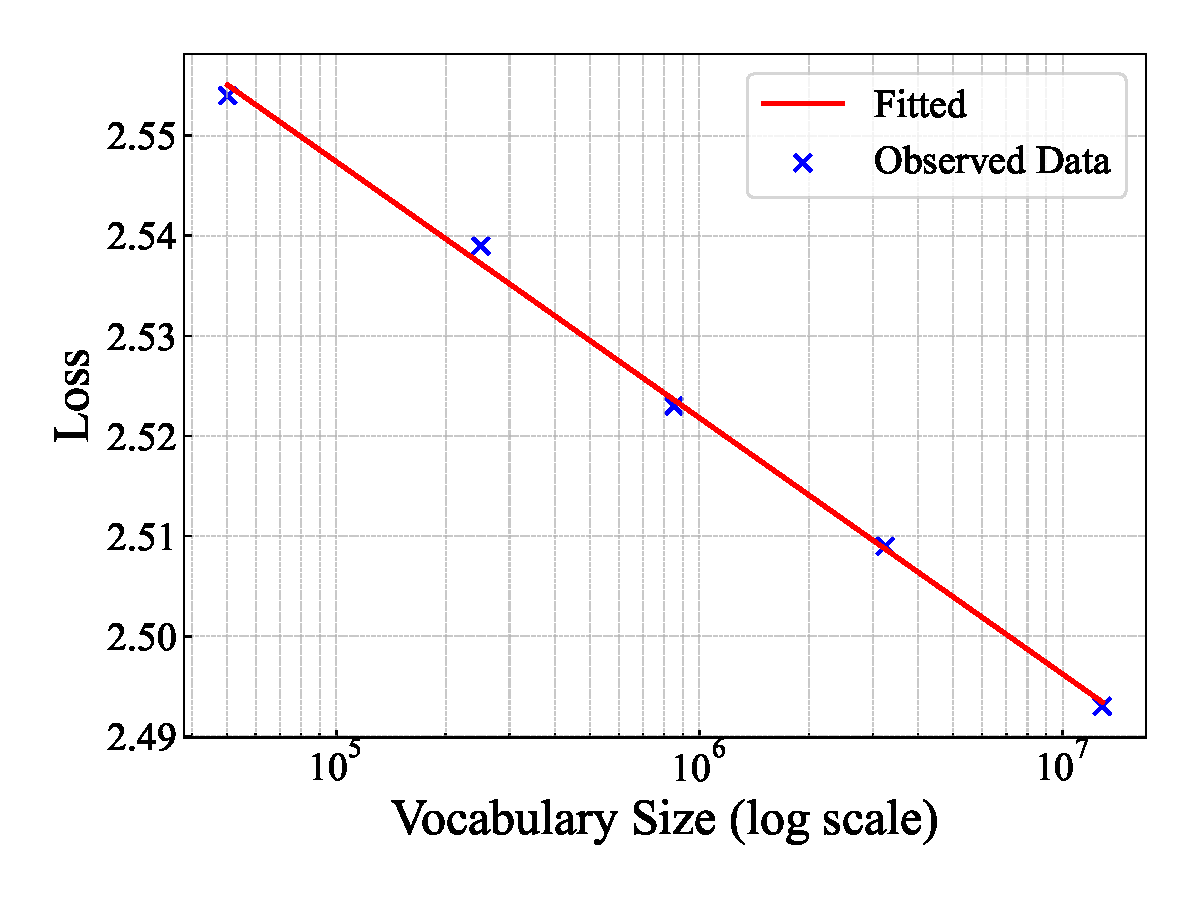
\includegraphics[width=0.8\linewidth]{figures/vocabsize_scaling_curve.pdf}
    \caption{Log-linear relationship is observed between vocabulary size $m$ and training loss $\mathcal{L}$, \ie $\mathcal{L}=2.6754-0.0256 \times\log_{10}{m}$. The values are collected with 500B tokens' training on OLMoE-1.3B models.}
    \label{fig:input_vocab_scaling}
\end{figure}

\begin{table}
\centering
\caption{Ablation study for the hierarchical design of over-encoding. The symbol `\cmark' on the $n$-gram column denotes $n$-gram token $x^{(-n)}$ is adopted. The experiments are conducted with $m=3.2\mathrm{M}$, and the metrics are reported after training on 50B tokens.}
\begin{tabular}{cccc|cccc}
\toprule
1-Gram & 2-Gram & 3-Gram & $k$ & Loss$\downarrow$ & PPL$\downarrow$ \\ \midrule
\cmark & \xmark & \xmark & - & 2.714 & 15.094  \\
\xmark & \cmark & \xmark & 1 & 2.785 & 16.205  \\ 
\cmark & \cmark & \xmark & 1 & \textbf{2.678} & \textbf{14.555}  \\
\midrule
\cmark & \cmark & \xmark & 4 & 2.670 & 14.447  \\
\cmark & \xmark & \cmark & 4 & 2.684 & 14.642  \\
\cmark & \cmark & \cmark & 4 & \textbf{2.667} & \textbf{14.394}  \\
\bottomrule
\end{tabular}
\label{tab:ablation_hierarchical_multigram}
\end{table}


\paragraph{What's Good for OE.}
We conducted extensive ablation studies on different configurations for the over-encoding. To ensure fairness, all configurations have the same number of embedding parameters. The results are shown in the \tabref{tab:over_enc_good_exps}. For simplification, we denote C-$i$ as configuration $i$ in the table.

We first validate that slicing the embedding table along the $d$ dimension yields further gains (comparing C-2, C-4, and C-5). Then, C-3 is constructed as a baseline, where we keep using one embedding table but scale up $m$ and scale down $d$. Such configuration also improves baseline but underperforms C-4 and C-5. We attribute this to the reduced memory access: configuration 4 accesses $2d_\text{model}$ embedding parameters while configuration 3 accesses only $1.5d_\text{model}$ per token. Moreover, we validate the benefits of enlarging $n$ from 2 to 3 by comparing C-5 and C-6. With longer-range dependencies introduced, C-6 further improves performance. Lastly, these tricks are then applied on a larger vocabulary with $m=12.8\mathrm{M}$ (comparing C-7 and C-8). We observe even larger gains comparing to experiments with $m=3.2\mathrm{M}$. Note that C-6 and C-8 meets our default OE implementation, \ie, OE-3.2M and OE-12.8M respectively, as described in \eqref{eq:oe_standard}. 



\begin{table}
\centering
\caption{Ablation study on hashing conflicts. Note the experiments are kept roughly the same vocabulary size, \ie $64V\approx3.218\mathrm{M}$. The metrics are reported after training with 50B tokens.}
\begin{tabular}{c|cccc}
\toprule
Model & Loss$\downarrow$ & PPL$\downarrow$ & Eval Loss$\downarrow$ & Eval PPL$\downarrow$ \\ \midrule
baseline & 2.714 & 15.094 & 3.094 & 22.060 \\
+$\mathbb{E}^{64V\times d}$ & 2.702 & 14.892 & 3.077 & 21.710\\
+$\mathbb{E}^{3.2\mathrm{M}\times d}$ & \textbf{2.678} & \textbf{14.555} & \textbf{3.054} & \textbf{21.202}\\
\bottomrule
\end{tabular}
\label{tab:ablation_hashing_conflicts}
\end{table}




\paragraph{What's Bad for OE.}
We also identify certain configurations that result in significant performance degradation and should avoid in practice. For this part of the experiments, due to the obvious performance drop, we report results after training on only 50B tokens, and simply use loss and perplexity as evaluation metrics. 

First, we validate the importance of hierarchical multi-gram tokens. As shown in \tabref{tab:ablation_hierarchical_multigram}, removing the 1-gram vocabulary and using only the 2-gram vocabulary leads to a significant performance drop. This may be due to conflicts in the lookup results of the 2-gram table when 1-gram information is absent, making it difficult for the model to disambiguate the current semantics. On the other hand, skipping the 2-gram tokens and using only 1-gram and 3-gram tokens still shows gains over the baseline but underperforms the proposed model using 1-, 2-, and 3-gram tokens together. Overall, we hypothesize that the model benefits from hierarchical encoding to handle conflicting entries in the embedding table, thereby accurately resolving semantics.

Another supporting observation is that when we deliberately introduce more encoding conflicts (by setting $m$ to be an exact multiple of $V$), the gains of over-encoding are significantly reduced, as shown in \tabref{tab:ablation_hashing_conflicts}. This observation also suggests that $m$ should set to a value coprime with $V$ to avoid such degeneration.


\subsection{Over-Tokenized Transformer}

In this section, we verify the effectiveness of over-tokenized transformer. We conduct the experiments on OLMoE-1.3B with 500B tokens' training. As MTP is less efficient for smaller models, our implementation has only one extra head predicting the next 2 token, and set the weight 0.1 for future token loss. Then, the over-tokenized transformer is constructed, combining OE-12.8M with MTP-DS, which we refer as OT-12.8M.

Results are shown in \tabref{tab:olmoe_mtp_oe}. 
Limited by model capacity, MTP shows no improvement, as well as its stronger verison MTP-DS. However, with over-encoding plugged, MTP-DS presents greater power. OT further improves the downstream metric by 1. 3\% compared to OE, although it slightly sacrifices the loss gains of OE. The detailed metrics are presented in Appendix~\ref{sec:appendix_detailed_olome_exps}.

\begin{table}
\centering
\caption{MTP Experiments on OLMoE-1.3B. The loss refers to the next one token prediction loss for MTP methods. Metric difference that improves baseline are marked blue while degrations are marked red.}
\resizebox{\columnwidth}{!}{
\begin{tabular}{l|lll}
\toprule
Model & Loss$\downarrow$ & Eval Loss$\downarrow$ & Downstream$\uparrow$ \\ 
\midrule
baseline & 2.554 & 2.924 & 0.510 \\
+MTP & 2.556 \scriptsize \textcolor{red}{+0.002} & 2.925 \scriptsize \textcolor{red}{+0.001} & 0.508 \scriptsize \textcolor{red}{-0.002} \\
+MTP-DS & 2.555 \scriptsize \textcolor{red}{+0.001} & 2.926 \scriptsize \textcolor{red}{+0.002} & 0.511 \scriptsize \textcolor{blue}{+0.001} \\
\hline
OE-12.8M & 2.472  & 2.862  & 0.524  \\
OT-12.8M & 2.481 \scriptsize \textcolor{red}{+0.009} & 2.869 \scriptsize \textcolor{red}{+0.007} & 0.537 \scriptsize \textcolor{blue}{+0.013} \\
\bottomrule
\end{tabular}
}
\label{tab:olmoe_mtp_oe}
\end{table}

\subsection{Speed Analysis}
We analyze training and inference speed for over-encoding in this section. To illustrate training efficiency, we show training throughputs in OLMoE experiments in Table~\ref{tab:training_throughputs}, where we run OE and baseline under the same hardware configurations. OE in OLMoE-7B yields more overhead as we did not carefully optimize engineering configurations. 

\begin{table}[h]
\centering
\begin{tabular}{lll}
\toprule
 & \textbf{OLMoE-1.3B} & \textbf{OLMoE-7B} \\
\midrule
Hardware & 32$\times$A100 & 64$\times$A100 \\
Baseline & 1.211 & 0.494 \\
+OE 12.8M & 1.155 \scriptsize -4.63\% & 0.453 \scriptsize-8.3\% \\
\bottomrule
\end{tabular}
\caption{Training throughputs for OE and baseline. We report average tokens per second in millions.}
\label{tab:training_throughputs}
\end{table}



\begin{table*}[h!]
\centering
\begin{tabular}{cc|rr|rr|rr}
\hline
\multirow{2}{*}{\textbf{Batch Size}} & \multirow{2}{*}{\textbf{Phase}} 
& \multicolumn{2}{c|}{\textbf{Dense-1B}} 
& \multicolumn{2}{c|}{\textbf{MoE-1B/7B}} 
& \multicolumn{2}{c}{\textbf{Dense-7B}} \\
\cline{3-8}
& & Baseline & OE-12.8M & Baseline & OE-12.8M & Baseline & OE-12.8M \\
\hline
\multirow{2}{*}{1} 
& Prefill & 20728.7 & 19446.4 & 6303.8 & 6189.0 & 6571.0 & 6499.9 \\
& Decode  &   136.2 &   126.6 &   28.2 &   27.9 &   65.1 &   63.3 \\
\hline

\multirow{2}{*}{8} 
& Prefill & 36907.5 & 35902.6 & 22297.3 & 22292.1 & - & - \\
& Decode  &   797.2 &   760.9 &  184.9 &  181.0 &  232.1 &  228.6 \\
\hline
\multirow{1}{*}{64} 
& Decode  & 1422.1 & 1407.4 &  860.3 &  826.7 & - & - \\
\hline
\end{tabular}
\caption{Inference speed for OE and baseline. The sequence length is fixed to 2048, and we report tokens per second for prefilling and decoding separately under various batchsizes. Settings that cause OOM are leave blank.}
\label{tab:inference_speed}
\end{table*}

\begin{table}[h!]
\centering
\begin{tabular}{lll}
\toprule
 & \textbf{OLMoE-1.3B} & \textbf{OLMoE-7B} \\
\midrule
baseline & 0.5409 & 2.3578 \\
+OE 12.8M & 0.5430 \scriptsize+0.38\% & 2.3662 \scriptsize+0.35\% \\
\bottomrule
\end{tabular}
\caption{GFLOPs per token in the forward pass.}
\label{tab:training_flops}
\end{table}

Theoretically, the additional flops introduced by OE is less than 0.5\% (as shown in the table below), as demonstrated in Table~\ref{tab:training_flops}. The overhead measured in the experiments should mainly be introduced by the all-to-all communication (which is proportional to the size of data parallel). And these communication overheads can be further optimized through engineering techniques in the future.

For inference efficiency, we test the prefill and decoding throughput on a single A100 GPU using the \texttt{transformers} library. For the OE models, the additional embedding parameters are offloaded to the CPU, \textbf{incurring no GPU memory overhead}. The numeric results are shown in Table~\ref{tab:inference_speed}. The impact of OE on inference throughput is negligible, especially for larger models or larger batch sizes. In contrast, the sparse parameters introduced by MoE face severe memory access bottlenecks during inference. A very large batch size is required for the MoE model to achieve the same throughput as a dense model with the same activated parameters. Considering that the model inference might be carried out on more cost-effective but less computationally powerful inference GPUs, the relative overhead of OE could be further reduced.

